\documentclass[journal]{IEEEtran}
\usepackage[brazil]{babel}
\usepackage[utf8]{inputenc}
\usepackage[pdftex]{graphicx}

\begin{document}
	
%Titulo do artigo
\title{Controle e supervisão de um sistema de caldeira simulado}

%Nomes dos autores
\author{Pedro Cézar Rodrigues Baltazar (402085)~Sergio Franco Sales Filho (414596)% <-this % stops a space
\thanks{A. 1, Universidade Federal do Ceará, Sobral, Brasil}% <-this % stops a space
\thanks{A. 2, Universidade Federal do Ceará, Sobral, Brasil}% <-this % stops a space
}

% The paper headers
\markboth{Controle de Caldeira - SOFTWARE EM TEMPO REAL}%
{Shell \MakeLowercase{\textit{et al.}}: Bare Demo of IEEEtran.cls for IEEE Journals}


% make the title area
\maketitle

% As a general rule, do not put math, special symbols or citations
% in the abstract or keywords.
\begin{abstract}
Utilizando um simulador feito em java de uma caldeira controlada via software, foi possível
fazer um programa em C que controlasse o sistema dessa caldeira, utilizando, principalmente, a biblioteca \textit{pthread}, que com
ela é possível criar \textit{threads} do zero, fazer controle de acesso de variáveis com
\textit{mutex} (implementado por meio de monitores), fazer medições de tempo de execução etc. Basicamente, na caldeira, há sensores
e atuadores que podem ser lidos e modificados utilizando o protocolo de comunicação exigido
pelo sistema.
\end{abstract}

% Note that keywords are not normally used for peerreview papers.
\begin{IEEEkeywords}
\textit{Thread}, caldeira, \textit{mutex}, C, atuadores, sensores.
\end{IEEEkeywords}

\IEEEpeerreviewmaketitle

\section{Introdução}

\IEEEPARstart{S}{istemas} de Tempo Real (STR) são sistemas que são elaborados com o propósito secundário, além
do propóstio principal do projeto, de que suas tarefas ou funções sejam executadas dentro
de certas requisições de tempo, como de período, de \textit{deadline} e de tempo de execução.
Assim, torna-se necessário que o sistema atenda a todas essas exigências, onde, muitas vezes
um mesmo processador/memórias são utilizados para a execução de todo o projeto, que, por sua vez, também
podem concorrer por esses recursos.

Portanto, é implementada a idéia do \textit{mutex}, que tem a função de bloquear posições da
memória especificadas no programa, para que outras \textit{threads} que concorrem com está
variável não possam acessá-las e causar possíveis problemas de cálculos que dependem do valor
desta variável. E, para a implementação do \textit{mutex}, foram utilizados monitores, que,
basicamente, são mecanismos de sincronização de \textit{threads} que são implementados no
programa na forma de módulos, onde todos os problemas relacionados com o acesso de variáveis
compartilhadas acontecem apenas dentro dos monitores, que garantem a segurança no momento
de acesso dessas variáveis.

Com isso, foi possível elaborar um programa em C que colhesse informações a respeito do
estado de funcionamento de uma caldeira (em simulação), bem como, enviasse valores de vazão ($kg/s$) e calor
($J/s$), dentre outros, para o controle deste estado de funcionamento. Assim, este trabalho
pretende demonstrar a utilização da biblioteca \textit{pthread} (linguagem C) na elaboração
de \textit{threads} e \textit{mutex} para controlar determinados parâmetros de funcionamento
de um sistema de aquecimento (caldeira), onde todos os processos acontecem dentro dos monitores,
contando com a comunicação (coleta e envio) entre o software e o sistema de atuadores e sensores da caldeira,
com os cálculos feitos relativos ao controle de temperatura, nível e vazões de água, com a disponibilização
das informações na tela e coleta da entrada pelo usuário do software e, por fim, com o registro das informações obtidas durante a exeução do programa em um
arquivo de \textit{log}.

\section{Metodologia}

\subsection{Sistema da Caldeira}
Para o sistema da caldeira, utilizando o software de simulação de aquecimento de uma caldeira, que possibilita
uma comunicação com o programa via LAN, utilizando o protocolo de comunicação entre caldeira e programa, onde
o programa pode enviar um pedido de valor de medição de um sensor ou enviar um valor para um atuador de
acordo com o protoclo correto. Para realizar a comunicação entre o simulador e o programa, iniciou-se o programa
em linha de comando como \textit{java -jar Aquecedor2021.jar \textless porta \textgreater}. Já para o início do programa criado,
após a compilação, foi executado o comando \textit{./controle-caldeira \textless ip-local-do-simulador\textgreater \vspace{1pt} \textless porta\textgreater}.

Da caldeira, é possível ler os sensores \textit{Ta} (temperatura ambiente), \textit{T} (temperatura na caldeira),
\textit{Ti} (temperatura da água não controlada de entrada do atuador), \textit{No} (temperatura da água de saída) e
\textit{H} (nível de água na caldeira). E, para o controle da caldeira, é possível configurar valores
para os atuadores \textit{Ni} (vazão de água de entrada de temperatura não controlada),
\textit{Q} (calor gerado pelo aquecedor), \textit{Na} (vazão de entrada de água a $80 ^{\circ} C$) e
\textit{Nf} (fluxo de água de saída para o esgoto).

Assim, com esses valores obtidos pelos sensores e a possibilidade de alteração dos atuadores,
foi possível configurar a caldeira para alcançar valores específicos de temperatura (\textit{T}) e de
nível de água (\textit{H}), utilizando equações que relacionam essas grandezas relativas ao sistema da caldeira.

Para o controle da temperatura na caldeira (\textit{T}) e do nível de água (\textit{H}), foi pedido como
entrada, no início da execução do programa (uma única vez), valores de temperatura de referência e de
nível de referência, respectivamente, inseridos pelo usuário.


\subsection{Medições de Tempo Real}
Já para a parte de medições de tempo real, que variam devido ao design do sotware (programação concorrente),
outras atividades do sistema e devido ao \textit{hardware}, foi medido o tempo de resposta, com mais de 10.000
amostras, da tarefa de controle de temperatura da caldeira, onde o $N_o$ foi variada mais de cinco vezes pela
interface do software do simulador. Para a medição do tempo de resposta, foi utilizado o relógio interno do
sistema operacional antes e depois do início da execução da \textit{thread} e, para armazenar os resultados,
foi utilizado um \textit{buffer} duplo (produtor/consumidor) que guarda os seus valores armazenados em um
arquivo \textit{.txt}, que posteriormente, foi utilizado no software \textit{MatLab} para um estudo
estatístico detalhado do tempo de execução desta tarefa, como será visto na próxima seção.

\section{Resultados e discussões}
Do sistema da caldeira, foi observado que existe um certo intervalo de tempo até os valores de temperatura
e de nível chegarem aos seus valores de referência, isso pode ser explicado dado que a temperatura da caldeira e o nível de água estão relacionados de
uma forma que quando qualquer uma das \textit{threads} (controle de temperatura ou controle de nível) entram
em ação, podem prejudicar ou ajudar a atuaçao da outra.

Já para a parte das medições de tempo real, foi possível obter o resultado de mais de 10.000 medições. Esse
resutado foi utilizado no \textit{MatLab} e foi feito doi gráficos: um gráfico de dispersão das amostras (na
ordem dos casos de teste) e um gráfico de histograma das mediçõs realizadas, como é possível observar na 
figura abaixo.

\begin{figure}[h]
	\centering
	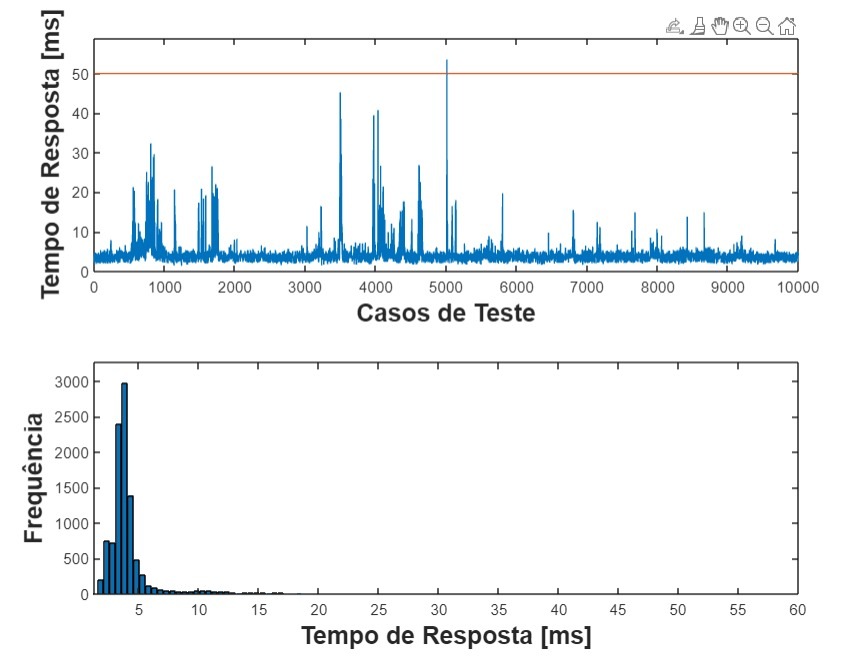
\includegraphics[width=3.5in]{Imagens/resultado.jpeg}	
	\caption{Gráfico com as medições realizadas, na ordem dos casos de teste.}
	\label{fig1}
\end{figure}

De acordo com a figura, é possível visualizar o valor médio do tempo de resposta de todos os casos de teste
(por volta de $50 \,ms$) e, também, no histograma, que a maior parte dos tempos de medição não passaram de 
$10 \,ms$, onde, a maior parte dos casos estão próximos dos $4 \,ms$ de tempo de execução.

%%%%%%%%%%%%%%%%%%%%%%%%%%%%%%%%%%%%%%%%%%%%%%%%5
%%%%%%%%%%%%%%%%%%%%%%%%%%%%%%%%%%%%%%%%%%%

\ifCLASSOPTIONcaptionsoff
  \newpage
\fi

\begin{thebibliography}{1}

\bibitem{IEEEhowto:romulo}
Oliveira, R. S. Fundamentos dos Sistemas de Tempo Real. Original registrado na Biblioteca Nacional. Primeira edição, revisão 3, outubro de 2018. ISBN-13: 9781728694047.

\end{thebibliography}

%%%%%%%%%%%%%%%%%%%%%%%%%%%%%%%%%%%%%%%%%
%Se tiver foto use essa forma
\begin{IEEEbiography}[{
\includegraphics[width=1in,height=1.25in,clip,keepaspectratio]{Imagens/Brasao_UFC.jpg}}]{Autores}
Universidade Federal do Ceará (UFC) - Campus Mucambinho
\end{IEEEbiography}


\end{document}